\documentclass[border=2pt]{standalone}
% Shared preamble for the standalone result plots (fig/src/*.tex).
% Compile:  tectonic -X compile fig/src/<name>.tex --outdir fig/src/out
% then copy fig/src/out/<name>.pdf over fig/<name>.pdf
%
% Palette matches the paper: wacvblue is main.tex's link colour, orange is xcolor's.
\usepackage{iftex}
\ifXeTeX
  \usepackage{fontspec}
  \setmainfont{texgyretermes}[Extension=.otf, UprightFont=*-regular,
    BoldFont=*-bold, ItalicFont=*-italic, BoldItalicFont=*-bolditalic]
\fi
\usepackage{pgfplots}
\pgfplotsset{compat=1.18}
\usepackage{amsmath}
\definecolor{wacvblue}{rgb}{0.21,0.49,0.74}
\pgfplotsset{
  resultaxis/.style={
    axis background/.style={fill=white},
    grid=major, ymajorgrids=true, xmajorgrids=false,
    grid style={gray!25, line width=0.3pt},
    tick align=outside, tick pos=left,
    label style={font=\small}, tick label style={font=\small},
    legend style={font=\small, draw=gray!50, fill=white, fill opacity=0.9,
                  text opacity=1, inner sep=2pt},
  },
  vidmark/.style={wacvblue, mark=*, thick, mark size=2.2pt},
  eegmark/.style={orange, mark=o, thick, dashed, mark size=2.2pt},
}

\begin{document}
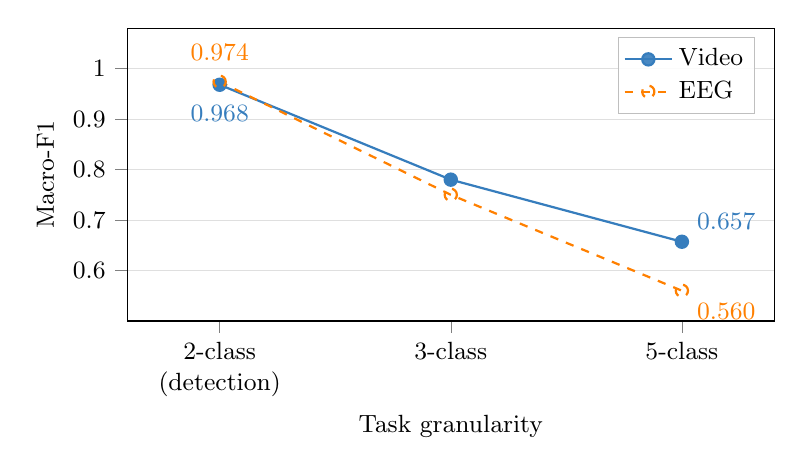
\begin{tikzpicture}
\begin{axis}[
  resultaxis,
  width=9.8cm, height=5.3cm,
  xlabel={Task granularity}, ylabel={Macro-F1},
  xtick={1,2,3},
  xticklabels={{2-class\\(detection)}, {3-class}, {5-class}},
  xticklabel style={align=center},
  xmin=0.6, xmax=3.4, ymin=0.50, ymax=1.08,
  ytick={0.6,0.7,0.8,0.9,1.0},
  legend pos=north east, legend cell align=left,
]
\addplot[vidmark] coordinates {(1,0.968) (2,0.780) (3,0.657)};
\addlegendentry{Video}
\addplot[eegmark] coordinates {(1,0.974) (2,0.750) (3,0.560)};
\addlegendentry{EEG}
% value labels, all anchored inside the axis box; the two detection points
% are close (0.968 vs 0.974), so they are split below/above.
\node[wacvblue, font=\small, anchor=north,      yshift=-4pt]             at (axis cs:1,0.968) {0.968};
\node[orange,   font=\small, anchor=south,      yshift=4pt]              at (axis cs:1,0.974) {0.974};
\node[wacvblue, font=\small, anchor=south west, xshift=2pt, yshift=1pt]  at (axis cs:3,0.657) {0.657};
\node[orange,   font=\small, anchor=north west, xshift=2pt, yshift=-1pt] at (axis cs:3,0.560) {0.560};
\end{axis}
\end{tikzpicture}
\end{document}
